\section{Durchführung der Aufgabe}

In diesem Kapitel beschreiben wir konkret, wie die Arbeit sich während meines Praxissemesters sich entwickelte. Die ersten zwei Wochen dienten als Einarbeitung und Einstieg. Nach dieser Phase bekam ich langsam und unter Betreuung mehr Verantwortung und mehr Freiheit, um die Aufgaben durchzuführen. In der folgenden Tabelle wird der Ablauf systematisch und undetailliert beschrieben. Im zweiten Teil dieses Kapitels geben wir eine ausführliche Beschreibung eines Projekts.

Bei WALLSEC hat jedes Projekt  einen festgelegten Aufbau. Dieser kann in den folgenden Punkten zusammengefasst werden:

\begin{enumerate} \label{Projektablauf}
    \item \textit{Kick-off Meeting} mit dem Kunden, um grundsätzliche Informationen über die Anwendung zu bekommen
    \item Definition des Testumfangs, wie Anmeldedaten, Rolle der Nutzer, \glsplural{Tenant} und mögliche Einschränkungen
    \item Durchführung von Tests nach einer vorgegebenen Checkliste
    \item Dokumentation der durchgeführten Tests, der gefundenen \glsplural{Schwachstelle} und Vorschläge zur Härtung der Anwendung
    \item Abschlussmeeting mit dem Auftraggebern, um die \glsplural{Schwachstelle} und deren Ausnutzung zu demonstrieren
\end{enumerate} 

\subsection{Wöchentliche Zusammenfassung meines Praxissemesters}

\begin{table}[H]
    \setstretch{1.0}
    \begin{tabularx}{\textwidth}{|c|X|}
    \toprule
    \multicolumn{2}{c}{\textbf{Auflistung der Aufgabe}} \\
    \midrule
    \multicolumn{1}{c}{\textbf{Woche}} & \multicolumn{1}{c}{\textbf{Aufgabeschreibung}} \\
    \hline
    1 - 2    & Einarbeitung:
                \begin{itemize}
                    \item Installation von einer virtuellen Maschine für die Testumgebungen
                    \item Einführung in der Arbeitsablauf der Firma
                    \item Einführung, Installation und Einstellungen von \gls{burp}
                    \item Einführung in ein laufendes Projekt, um über das Ablauf- und Dokumentationsverfahren zu lernen
                    \item Durchführung und Wiederholungen von einigen Tests, um mich an den gegebenen Tools zu gewöhnen
                    \item Teilnahme an einem Abschlussmeeting des laufenden Projekts, um das Verfahren und den Ablauf des Kundenkontakts kennenzulernen und später zu wiederholen
                \end{itemize} \\
        \hline

    3 - 4       &  Start, Durchführung und Abschluss eines neuen Pentesting-Projekts an einer Versicherungsanwendung mit den obigen beschriebenen Schritten (\ref{Projektablauf})  \\ 
    
        \hline
    
    5 - 6       & Weiterarbeit an der Installation, Einstellungen und Nutzung der Tools \gls{TheHive} und \gls{Cortex}. Bereitstellung von Skripts zum Herunterladen von statistischen Daten der Anwendungen und zur Automatisierung deren Nutzung.  \\ 
    
        \hline
    
    7 - 8      &  Start, Durchführung und Abschluss eines neuen Pentesting-Projekts an einer Marketing-Webanwendung mit den oben beschriebenen Schritten (\ref{Projektablauf}) \\

        \hline

    9 - 10  &  Start, Durchführung und Abschluss eines neuen Pentesting-Projekts in Netzwerk-Umgebungen mit den oben beschriebenen Schritten (\ref{Projektablauf}). Die durchgeführten Tests konzentrierten sich auf die Sicherheit eines Netzwerks in einer Cloud-Umgebung. Für dieses Projekt spielten die Tools \gls{nmap} und \gls{scout} eine wichtige Rolle, da das Ziel war, Hosts, Dienste und ihre Einstellungen und \gls{Schwachstelle}n zu erkennen \\

    \hline

    11  	&  Start, Durchführung und Abschluss eines Pentestings von einer umfangreichen Webanwendung mit verschiedenen \glsplural{Tenant} und Nutzerrollen für die Verwaltung von Business-Prozessen. \\

    \hline

    11 - 14 &  Start, Durchführung und Abschluss eines Pentestings wessen Aufbau auf \glsfirst{http} und \gls{graphql} basiert war. Da diese beiden Technologien mir ganz neu waren, beschäftigte ich mich intensiv damit, sie in ihrem Aufbau und möglichen \glsplural{Schwachstelle} zu erforschen. \\

    \hline

    15     &  Weiterarbeit an das Projekt mit \gls{TheHive} und \gls{Cortex}, indem verschiedene \glsplural{Skript} in \gls{python} geschrieben wurden, um Kommunikation zwischen \gls{TheHive} und \gls{Cortex} und anderen Anwendungen aufzubauen. Diese \glsplural{Skript} sollten auch Daten zu den Anwendungen importieren und exportieren.\\

    
%    \hline

%    19 - 20      &  xxxxxx \\
       \bottomrule
    \end{tabularx}
\end{table}

\begin{table}[H]
    \setstretch{1.0}
    \begin{tabularx}{\textwidth}{|c|X|}
    \toprule
    \multicolumn{2}{c}{\textbf{Auflistung der Aufgabe}} \\
    \midrule
    \multicolumn{1}{c}{\textbf{Woche}} & \multicolumn{1}{c}{\textbf{Aufgabeschreibung}} \\
    \hline
 
    16 - 17 &  Start, Durchführung und Abschluss eines neuen Pentesting-Projekts an einer Webanwendung mit den oben beschriebenen Schritten (\ref{Projektablauf}). Der Kern dieser Anwendung ist die Erstellung und Verwaltung von Lieferkette-Prozessen von seits der Anbieter und der Verkäufer. Bei diesem Projekt war der Test darauf fokussiert, die festgelegten Schritte der Lieferkette zu erkennen und, als potentieller Angreifer, diese Schritte willkürlich zu steuern. \\
    
    \hline

    18     &  Das Projekt dieser Woche war eine Fortsetzung desjenigen von Woche 15. Der Kunde hat andere Teile der Anwendung zur Verfügung gestellt, sodass wir ihre Sicherheit überprüfen können. Die durchgeführten Tests konzentrierten auf strukturellen Ebenen der Anwendung, besonders auf der Herstellung von Verbindung mit \glsplural{Websocket}. \\
    \hline

    19     &  Diese Woche war eine Fortsetzung an das Projekt von Woche 15. Hier wurde der Skript bis zu Ende geschrieben und bezüglich der Anmeldeart an der Umgebung des Beauftragter angepasst. \\
    \hline

    \textbf{20}     &  \textbf{Das Projekt diese Woche war eine klassische Webanwendung für Pentesting. Die Besonderheit bei diesem Projekt war meine Beteiligung an drei letzten Schritten: Durchführung, Dokumentation und Abschlussmeeting mit dem Auftraggeber. Bei den vorherigen Projekten bekam ich ständig Hinweise von meinem Betreuer in der Firma. Diesmal gab er mir völlig die Kontrolle über diese drei erwähnte Schritte. Ich war sicher nicht allein und konnte immer Fragen zu den Punkten stellen, wo ich mich immer noch unsicher fühlte. Vor der endgültigen Abgabe machten wir zusammen einen Review, um sicher zu sein, dass es an nichts fehlte. Ich kann diese Woche als wichtigen Zeitpunkt für meinen Karrierelaufbahn klassifizieren: vor ungefähr vier Monaten war ich ein fast erfahrungsloser Praktikant und danach wurde mir vertraut, fast selbständig ein Penetration-Testing durchzuführen.}  \\

    \hline

    21     &  TBD \\

    \hline

    22     &  TBD \\

    \hline

    23     &  TBD \\

    \hline

    24     &  TBD \\

    \hline

    25, 26, 27 &  Vertraglicher vereinbarter Urlaub. Diese Zeit benutzte ich, um dieses Bericht zu schreiben und zu verbessern. \\

    \hline

       \bottomrule
    \end{tabularx}
\end{table}


   



\subsection{Ausführliche Beschreibung eines Penetration Testing innerhalb des Praxissemesters}

Vor der Durchführung eines jeden Tests sind WALLSEC und ihre Mitarbeiter dazu verpflichtet, eine Vertraulichkeitserklärung zu unterschreiben. Es dürfen Informationen weder über die Firma noch über die verwendeten Methoden dürfen in irgendeiner Form veröffentlicht werden. Aus diesem Grund werden die hier demonstrierten Methoden und Tests in der Test- und Lernumgebung \glsfirst{dvwa} gezeigt. In den realen Tests verwenden wir ähnliche Methoden, manchmal mit mehr oder weniger Details, um die Sicherheit der Anwendungen zu überprüfen. 

Da dieses Thema zu umfangreich für den Zweck dieses Berichts ist, demonstrieren wir in den nächsten zwei Unterkapiteln nur einige Methoden, die wir verwenden, um die Zielanwendung in ihrer Struktur zu prüfen und auszunutzen.

\subsubsection{Sammlung von Informationen über das Zielsystem}

Obwohl jede Webanwendung ihre eigenen Eingenschaften und Ziele hat, besitzen fast alle eine ähnliche Struktur und Aufbau. Bei jedem Test fangen wir damit an, diese gemeinsame Struktur zu erkennen, indem wir nach öffentlichen Informationen suchen. Viele kritische Informationen, wie Username, Passwörter, Versionen, Systemen verbundenen IP-Adressen, lassen sich nach einer Online-Suche finden. Auch mit eingebauten Tools eines Betriebssystems können wir auf solche Informationen zugreifen. Dieses Verfahren nennen wir Banner Grabbing. Das folgende Bild zeigt ein Beispiel von einer einfachen Durchführung von Banner Grabbing:

\begin{figure}[H]
    \centering
    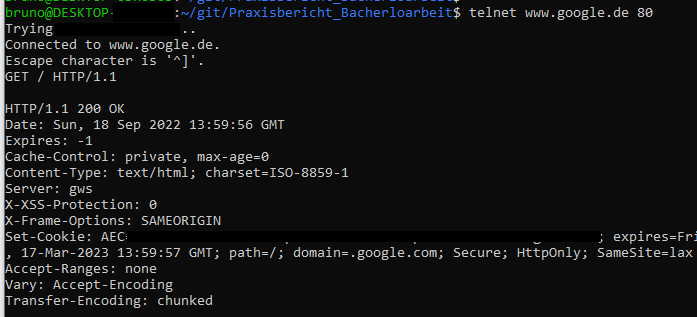
\includegraphics[width=0.5\textwidth]{/home/bruno/git/Praxisbericht_Bacherloarbeit/Praxissemester/assets/banner_grabbing.png}
    \caption{Banner Grabbing mithilfe vom Tool telnet}
    \centering
\end{figure}

Eine Webanwendung ist eine Gruppierung von verschiedenen Verzeichnissen. Jedes Verzeichnis soll dem Nutzer eine Information oder Interaktion anbieten. Manche sind aber nicht für Nutzer gedacht, sondern dienen zur Verwaltung von Einstellungen. Da solche Verzeichnisse nicht direkt aufrufbar sind, benutzen wir andere Methoden, um zu finden, was die Entwickler im Hintergrund beibehalten wollten. Es gibt verschiedene Tools, die mithilfe von sogenannten \textit{wordlists}, viele Anfragen an eine Anwendung schicken, um herauszufinden, was nicht direkt von dem Browser aufrufbar ist. Solche \textit{wordlists} sind Textdateien, die häufig verwendete Wörter für Webanwendungen, Nutzername oder Passwörter beinhalten. Da viele Webanwendungen ähnliche Strukturen haben, ist auch meistens erwartet, dass gewöhnliche Wörter zu finden sind. Das nächste Beispiel zeigt uns, dieses Entdeckungsverfahren auf unserem Ziel, \gls{dvwa} Tool. Hier benutzen wir das Tool \gls{dirb}, um herauszufinden, welche Verzeichnisse in dieser Anwendung existieren. In diesem Fall werden verschiedene Anfragen geschickt, jede mit einem verschiedenen Wort, um zu sehen, welche positive Antworten liefern. Das folgende Bild zeigt die Durchführung und das Ergebnis des Scanverfahrens mithilfe des Tools \gls{dirb}:

\begin{figure}[H]
    \centering
    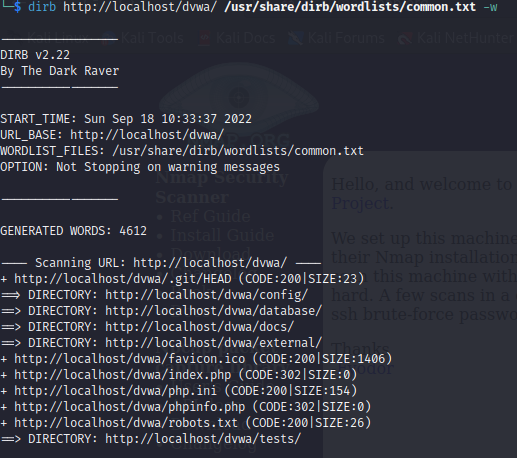
\includegraphics[width=0.5\textwidth]{/home/bruno/git/Praxisbericht_Bacherloarbeit/Praxissemester/assets/dirb.png}
    \caption{Brute force Scan für Verzeichnisentdeckung}
    \centering
\end{figure}

Der nächste Schritte wäre eine manuelle Analyse des entdeckten Materials, um zu prüfen, ob sensitive Informationen ausgeliefert wurden. Falls ja, würden wir dann versuchen diese \gls{Schwachstelle}, zu erkennen und auszunutzen.

Ein Netzwerk-Scan ist auch eine häufig verwendete Methode, um Dienste innerhalb des zu testenden Zielsystems zu finden. Dieser Scan schickt verschiedene Anfragen an das Ziel und so können wir die Reaktion des Zielsystems beobachten. Während wir uns bei dem ersten Scan auf die Webanwendung fokussierten, bearbeiten wir hier eine Ebene, die nicht für die gewöhnliche Nutzung gedacht ist. Unser Fokus liegt auf dem Server, wo die Anwendung läuft. Dafür testen wir die sogenannten \glsplural{port}. Aus diesem Scan lassen sich meistens viele nützliche Informationen herausfiltern, wie z.B. das Betriebssystems, auf dem die Webanwendung läuft, Name und Versionen der existierenden Dienste. Mit diesen Informationen ist dann es möglich zielgerichtete Angriffe vorzubereiten, um \glsplural{Schwachstelle} auszunutzen.

Das nächste Bild zeigt das Ergebnis der Durchführung von \gls{nmap} gegen das Testziel \textit{scanme.nmap.org}:

\begin{figure}[H]
    \centering
    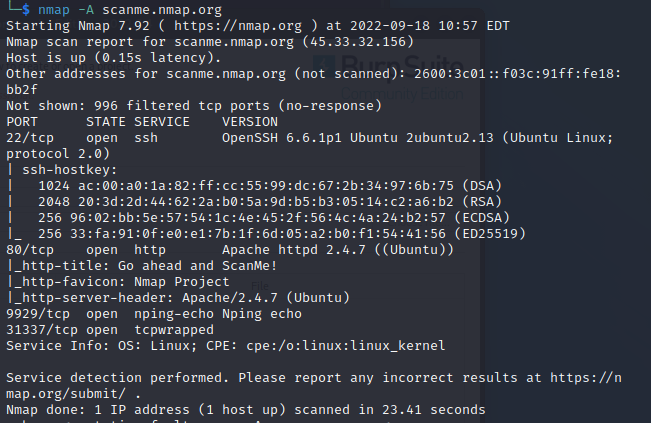
\includegraphics[width=0.5\textwidth]{/home/bruno/git/Praxisbericht_Bacherloarbeit/Praxissemester/assets/nmap.png}
    \caption{Brute force Scan für Verzeichnisentdeckung}
    \centering
\end{figure}

Aus diesem Scan erfahren wir welches Betriebssystem und welche Version die Webanwendung benutzt. Auch wenn solche Versionen gegen Angriffe geschützt sind, ist es unsere Aufgabe den Kunden zu informieren, dass sensitive Informationen für alle sichtbar sind. Ein böswilliger Nutzer könnte diese Informationen nutzen, um eine \glsplural{Schwachstelle} in dieser Anwendungen zu entdecken und diese auszunutzen.

\subsubsection{Ausnutzung der Zielanwendung}

Nachdem die vorherigen Scans durchgeführt und öffentliche Serverseite-Informationen gesammelt wurden, fangen wir mit den Tests auf der Webanwendung an. In diesem Fall ist es unser Ziel zu wissen, welche versteckten Daten oder unerlaubten Aktionen ein Angreifer durchführen kann, um die \gls{CIA} der Anwendung zu verletzen. Für die folgenden Tests benutzen wir unter anderem auch das Tool \gls{burp}.

Unser erster Test soll überprüfen, ob es möglich ist, in ein Eingabefeld Daten einzutragen und das normale Verhalten der Anwendung zu ändern. Wir versuchen eigenen Code hinzuzufügen und wenn uns das gelingt, fügen wir weiteren Code hinzu, um Daten von Nutzer zu stehlen oder das normale Verhalten der Anwendung zubeschädigen. Wir prüfen hier, ob die Anwendung gegen \glsfirst{xss} anfällig ist. Um diesen Test durchzuführen, fügen wir erwartete Daten hinzu, um das Verhalten der Anwendung zu beobachten. Nachdem wir das normale Verhalten erkannt haben, versuchen wir eigenen Code hinzufügen und beobachten, ob wir die Anwendung ausnutzen können. 

\begin{figure}[H]
    \centering
    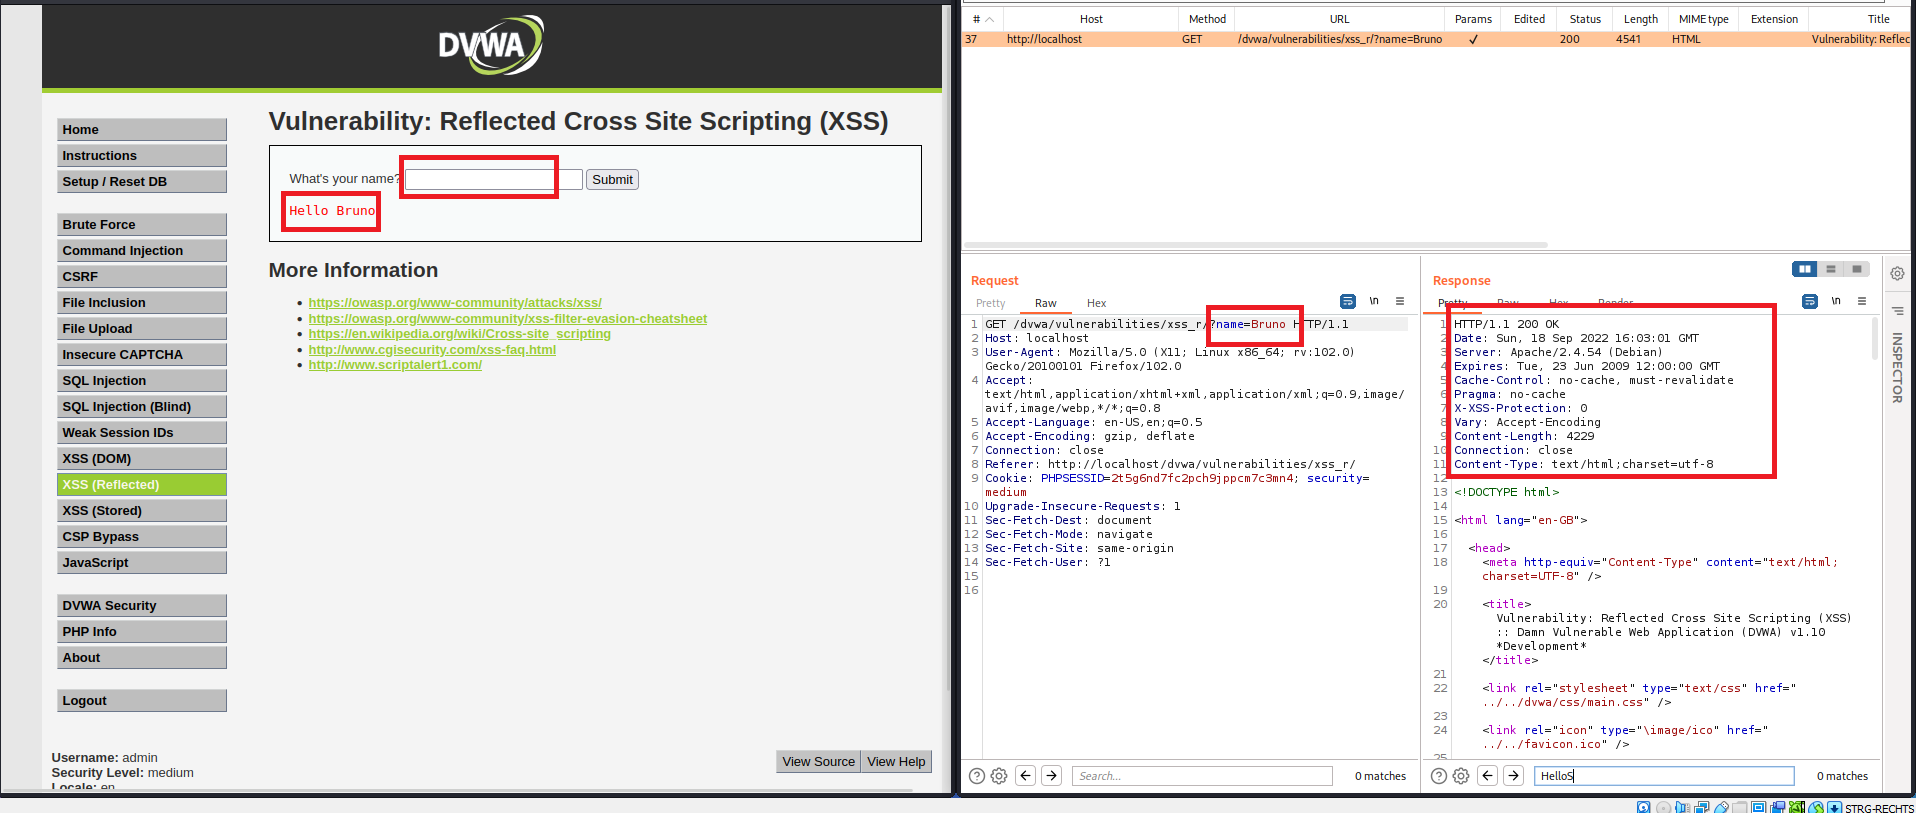
\includegraphics[width=0.8\textwidth]{/home/bruno/git/Praxisbericht_Bacherloarbeit/Praxissemester/assets/xssnormal.png}
    \caption{Beobachtung der Anwendung unter normale Nutzung}
    \label{fig:xssnormal}
    \centering
\end{figure}

Abbildung \ref{fig:xssnormal} zeigt den ersten Test. Aus dieser Aufnahme der Anfrage können wir sehen, dass die Nutzereingabe direkt in dem Browser stattfindet. In der Antwort sehen wir Informationen über den Aufbau der Anwendung und wie sie auf unsere Anfrage reagiert. Auf dem nächsten Bild versuchten wir bösartigen Code hinzuzufügen, um den normalen Ablauf der Anwendung zu verletzen. Dafür verwendeten wir \gls{javascript} Code. Wir konnten unseren Code direkt in die Anwendung, in einen selbst gebastelte Request oder in \gls{burp} eingeben:

\begin{figure}[H]
    \centering
    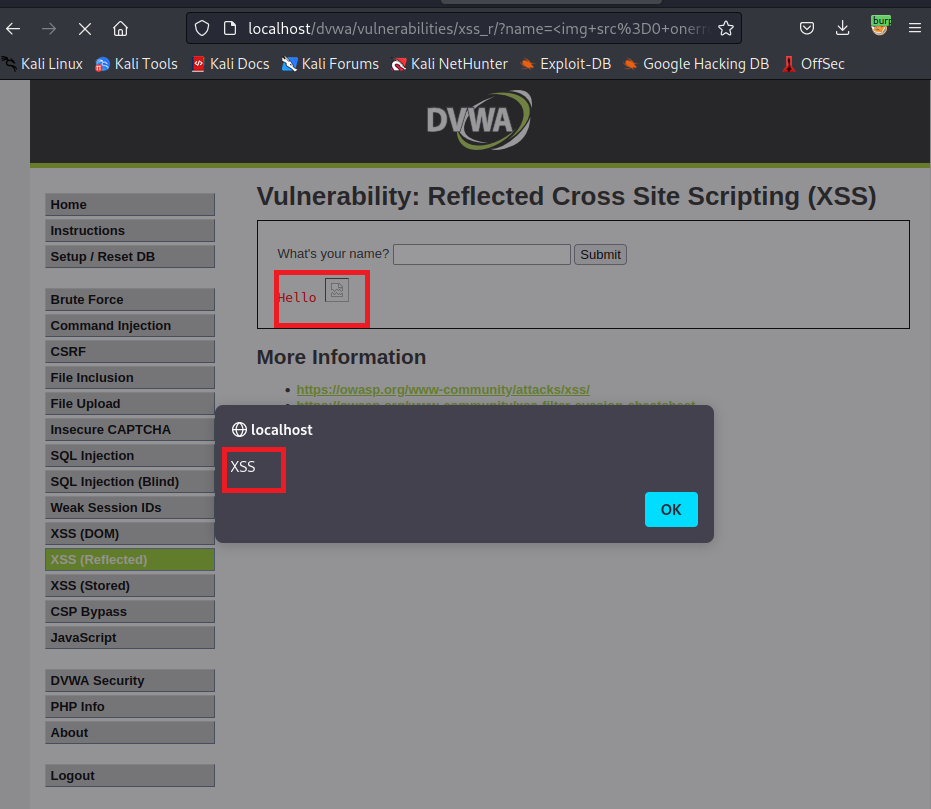
\includegraphics[width=0.8\textwidth]{/home/bruno/git/Praxisbericht_Bacherloarbeit/Praxissemester/assets/xss.png}
    \caption{Einführung vom bösartigem Code und Beobachtung der Reaktion der Anwendung.}
    \label{fig:xssexecuted}
    \centering
\end{figure}

Für diesen Test haben wir den Code \textit{<img src=0 onerror='alert(``XXS'')'\textbackslash>} hinzugefügt. Das Ziel dieses Codes ist ein nicht existierendes Bild hinzuzufügen, um einen absichtlichen Fehler zu provozieren. Dieser Fehler zeigt ein kleines Fenster in der Anwendung mit dem Text ```XSS'''. Eine geschützte Anwendung würde entweder den Code und ihren Zeichen ``< >'' ignorieren oder diese zu anderen übersetzen. Es kann auch sein, dass die Anwendung dem Nutzer zeigt, dass die eingegebenen Zeichen nicht erlaubt nicht. Aus dem Bild sehen wir aber, dass die Anwendung alle Zeichen akzeptiert und sogar erlaubt, dass der Code ausgeführt wird. Aus dieser Situation hätten wir einen \glsfirst{pof}, dass die Anwendung gegen diese Art von Angriff anfällig ist.


\subsubsection{Kundebericht}

Je nachdem wie lange das Projekt läuft, können wir mehr oder weniger zeitintensive Tests durchführen. Am Ende des Projekts präsentieren wir dem Auftraggeber in einem Meeting unser Ergebnis und liefern einen Bericht mit detaillierten Informationen über die gefundenen \glsplural{Schwachstelle} und die dazu verwendeten Methoden. Dieses Bericht wird so geschrieben, dass die Nichtfachleute es verstehen können. 

In den ersten Abschnitten erklären wir mit wenigen technischen Begriffen, welche Tests durchgeführt wurden. In den folgenden Kapiteln erklären wir mit mehr Einzelheiten und technischen Details, wie wir zu unserem Ergebnis kamen. Anschließend geben wir Vorschläge für die Verbesserung der Sicherheit der Webanwendung und zum Schluss geben wir mithilfe von \gls{CVSS} oder einer anderen von dem Kunden ausgewählter Metrik eine allgemeine Bewertung.
